\documentclass[twoside]{book}

% Packages required by doxygen
\usepackage{fixltx2e}
\usepackage{calc}
\usepackage{doxygen}
\usepackage{graphicx}
\usepackage[utf8]{inputenc}
\usepackage{makeidx}
\usepackage{multicol}
\usepackage{multirow}
\PassOptionsToPackage{warn}{textcomp}
\usepackage{textcomp}
\usepackage[nointegrals]{wasysym}
\usepackage[table]{xcolor}

% Font selection
\usepackage[T1]{fontenc}
\usepackage{mathptmx}
\usepackage[scaled=.90]{helvet}
\usepackage{courier}
\usepackage{amssymb}
\usepackage{sectsty}
\renewcommand{\familydefault}{\sfdefault}
\allsectionsfont{%
  \fontseries{bc}\selectfont%
  \color{darkgray}%
}
\renewcommand{\DoxyLabelFont}{%
  \fontseries{bc}\selectfont%
  \color{darkgray}%
}
\newcommand{\+}{\discretionary{\mbox{\scriptsize$\hookleftarrow$}}{}{}}

% Page & text layout
\usepackage{geometry}
\geometry{%
  a4paper,%
  top=2.5cm,%
  bottom=2.5cm,%
  left=2.5cm,%
  right=2.5cm%
}
\tolerance=750
\hfuzz=15pt
\hbadness=750
\setlength{\emergencystretch}{15pt}
\setlength{\parindent}{0cm}
\setlength{\parskip}{0.2cm}
\makeatletter
\renewcommand{\paragraph}{%
  \@startsection{paragraph}{4}{0ex}{-1.0ex}{1.0ex}{%
    \normalfont\normalsize\bfseries\SS@parafont%
  }%
}
\renewcommand{\subparagraph}{%
  \@startsection{subparagraph}{5}{0ex}{-1.0ex}{1.0ex}{%
    \normalfont\normalsize\bfseries\SS@subparafont%
  }%
}
\makeatother

% Headers & footers
\usepackage{fancyhdr}
\pagestyle{fancyplain}
\fancyhead[LE]{\fancyplain{}{\bfseries\thepage}}
\fancyhead[CE]{\fancyplain{}{}}
\fancyhead[RE]{\fancyplain{}{\bfseries\leftmark}}
\fancyhead[LO]{\fancyplain{}{\bfseries\rightmark}}
\fancyhead[CO]{\fancyplain{}{}}
\fancyhead[RO]{\fancyplain{}{\bfseries\thepage}}
\fancyfoot[LE]{\fancyplain{}{}}
\fancyfoot[CE]{\fancyplain{}{}}
\fancyfoot[RE]{\fancyplain{}{\bfseries\scriptsize Generated on Sun May 3 2015 16\+:07\+:32 for Arguments library by Doxygen }}
\fancyfoot[LO]{\fancyplain{}{\bfseries\scriptsize Generated on Sun May 3 2015 16\+:07\+:32 for Arguments library by Doxygen }}
\fancyfoot[CO]{\fancyplain{}{}}
\fancyfoot[RO]{\fancyplain{}{}}
\renewcommand{\footrulewidth}{0.4pt}
\renewcommand{\chaptermark}[1]{%
  \markboth{#1}{}%
}
\renewcommand{\sectionmark}[1]{%
  \markright{\thesection\ #1}%
}

% Indices & bibliography
\usepackage{natbib}
\usepackage[titles]{tocloft}
\setcounter{tocdepth}{3}
\setcounter{secnumdepth}{5}
\makeindex

% Hyperlinks (required, but should be loaded last)
\usepackage{ifpdf}
\ifpdf
  \usepackage[pdftex,pagebackref=true]{hyperref}
\else
  \usepackage[ps2pdf,pagebackref=true]{hyperref}
\fi
\hypersetup{%
  colorlinks=true,%
  linkcolor=blue,%
  citecolor=blue,%
  unicode%
}

% Custom commands
\newcommand{\clearemptydoublepage}{%
  \newpage{\pagestyle{empty}\cleardoublepage}%
}


%===== C O N T E N T S =====

\begin{document}

% Titlepage & ToC
\hypersetup{pageanchor=false,
             bookmarks=true,
             bookmarksnumbered=true,
             pdfencoding=unicode
            }
\pagenumbering{roman}
\begin{titlepage}
\vspace*{7cm}
\begin{center}%
{\Large Arguments library \\[1ex]\large 1.\+0.\+0 }\\
\vspace*{1cm}
{\large Generated by Doxygen 1.8.8}\\
\vspace*{0.5cm}
{\small Sun May 3 2015 16:07:32}\\
\end{center}
\end{titlepage}
\clearemptydoublepage
\tableofcontents
\clearemptydoublepage
\pagenumbering{arabic}
\hypersetup{pageanchor=true}

%--- Begin generated contents ---
\chapter{Namespace Index}
\section{Namespace List}
Here is a list of all documented namespaces with brief descriptions\+:\begin{DoxyCompactList}
\item\contentsline{section}{\hyperlink{namespace_arguments_library}{Arguments\+Library} }{\pageref{d5/d40/namespace_arguments_library}}{}
\item\contentsline{section}{\hyperlink{namespace_arguments_library_1_1_builders}{Arguments\+Library.\+Builders} }{\pageref{d7/d39/namespace_arguments_library_1_1_builders}}{}
\item\contentsline{section}{\hyperlink{namespace_arguments_library_1_1_exceptions}{Arguments\+Library.\+Exceptions} }{\pageref{dc/daa/namespace_arguments_library_1_1_exceptions}}{}
\end{DoxyCompactList}

\chapter{Hierarchical Index}
\section{Class Hierarchy}
This inheritance list is sorted roughly, but not completely, alphabetically\+:\begin{DoxyCompactList}
\item \contentsline{section}{Arguments\+Library.\+Builders.\+Argument\+Builder$<$ T $>$}{\pageref{d0/d6c/class_arguments_library_1_1_builders_1_1_argument_builder_3_01_t_01_4}}{}
\item \contentsline{section}{Arguments\+Library.\+Arguments}{\pageref{d0/d10/class_arguments_library_1_1_arguments}}{}
\item \contentsline{section}{Arguments\+Library.\+Command\+Line}{\pageref{db/d18/class_arguments_library_1_1_command_line}}{}
\item Exception\begin{DoxyCompactList}
\item \contentsline{section}{Arguments\+Library.\+Exceptions.\+Arguments\+Exception}{\pageref{d7/df5/class_arguments_library_1_1_exceptions_1_1_arguments_exception}}{}
\begin{DoxyCompactList}
\item \contentsline{section}{Arguments\+Library.\+Exceptions.\+Parse\+Exception}{\pageref{da/dd1/class_arguments_library_1_1_exceptions_1_1_parse_exception}}{}
\item \contentsline{section}{Arguments\+Library.\+Exceptions.\+Setup\+Exception}{\pageref{d1/d04/class_arguments_library_1_1_exceptions_1_1_setup_exception}}{}
\end{DoxyCompactList}
\end{DoxyCompactList}
\item \contentsline{section}{Arguments\+Library.\+Builders.\+Option\+Builder}{\pageref{d0/d9e/class_arguments_library_1_1_builders_1_1_option_builder}}{}
\end{DoxyCompactList}

\chapter{Class Index}
\section{Class List}
Here are the classes, structs, unions and interfaces with brief descriptions\+:\begin{DoxyCompactList}
\item\contentsline{section}{\hyperlink{class_arguments_library_1_1_builders_1_1_argument_builder_3_01_t_01_4}{Arguments\+Library.\+Builders.\+Argument\+Builder$<$ T $>$} \\*Fluent interface provider for building \hyperlink{class_arguments_library_1_1_arguments}{Arguments} }{\pageref{d0/d6c/class_arguments_library_1_1_builders_1_1_argument_builder_3_01_t_01_4}}{}
\item\contentsline{section}{\hyperlink{class_arguments_library_1_1_arguments}{Arguments\+Library.\+Arguments} \\*\hyperlink{class_arguments_library_1_1_arguments}{Arguments} Library entry point }{\pageref{d0/d10/class_arguments_library_1_1_arguments}}{}
\item\contentsline{section}{\hyperlink{class_arguments_library_1_1_exceptions_1_1_arguments_exception}{Arguments\+Library.\+Exceptions.\+Arguments\+Exception} \\*This is a base layer exception for \hyperlink{class_arguments_library_1_1_arguments}{Arguments} library exceptions }{\pageref{d7/df5/class_arguments_library_1_1_exceptions_1_1_arguments_exception}}{}
\item\contentsline{section}{\hyperlink{class_arguments_library_1_1_command_line}{Arguments\+Library.\+Command\+Line} }{\pageref{db/d18/class_arguments_library_1_1_command_line}}{}
\item\contentsline{section}{\hyperlink{class_arguments_library_1_1_builders_1_1_option_builder}{Arguments\+Library.\+Builders.\+Option\+Builder} \\*Fluent interface provider for building Options }{\pageref{d0/d9e/class_arguments_library_1_1_builders_1_1_option_builder}}{}
\item\contentsline{section}{\hyperlink{class_arguments_library_1_1_exceptions_1_1_parse_exception}{Arguments\+Library.\+Exceptions.\+Parse\+Exception} \\*Exception thrown during \hyperlink{class_arguments_library_1_1_arguments}{Arguments} parse phase when invalid command line input is detected }{\pageref{da/dd1/class_arguments_library_1_1_exceptions_1_1_parse_exception}}{}
\item\contentsline{section}{\hyperlink{class_arguments_library_1_1_exceptions_1_1_setup_exception}{Arguments\+Library.\+Exceptions.\+Setup\+Exception} \\*Exception thrown during \hyperlink{class_arguments_library_1_1_arguments}{Arguments} setup phase when invalid setup is detected }{\pageref{d1/d04/class_arguments_library_1_1_exceptions_1_1_setup_exception}}{}
\end{DoxyCompactList}

\chapter{Namespace Documentation}
\hypertarget{namespace_arguments_library}{\section{Package Arguments\+Library}
\label{namespace_arguments_library}\index{Arguments\+Library@{Arguments\+Library}}
}
\subsection*{Namespaces}
\begin{DoxyCompactItemize}
\item 
package \hyperlink{namespace_arguments_library_1_1_builders}{Builders}
\item 
package \hyperlink{namespace_arguments_library_1_1_exceptions}{Exceptions}
\end{DoxyCompactItemize}
\subsection*{Classes}
\begin{DoxyCompactItemize}
\item 
class {\bfseries Argument$<$ T $>$}
\begin{DoxyCompactList}\small\item\em Option argument representation. It is internal class, to use it, see Argument\+Builder$<$\+T$>$.  \end{DoxyCompactList}\item 
class \hyperlink{class_arguments_library_1_1_arguments}{Arguments}
\begin{DoxyCompactList}\small\item\em \hyperlink{class_arguments_library_1_1_arguments}{Arguments} Library entry point \end{DoxyCompactList}\item 
class \hyperlink{class_arguments_library_1_1_command_line}{Command\+Line}
\item 
class {\bfseries Converter}
\begin{DoxyCompactList}\small\item\em Converter helps with conversion of strings to desired types. \end{DoxyCompactList}\item 
class {\bfseries Help\+Text\+Generator}
\item 
class {\bfseries Option}
\begin{DoxyCompactList}\small\item\em \hyperlink{class_arguments_library_1_1_arguments}{Arguments} option representation See Option\+Builder to access it.  \end{DoxyCompactList}\item 
class {\bfseries Option\+Alias}
\item 
class {\bfseries Parser}
\begin{DoxyCompactList}\small\item\em This class is used for processing command line input arguments. \end{DoxyCompactList}\end{DoxyCompactItemize}

\hypertarget{namespace_arguments_library_1_1_builders}{\section{Package Arguments\+Library.\+Builders}
\label{namespace_arguments_library_1_1_builders}\index{Arguments\+Library.\+Builders@{Arguments\+Library.\+Builders}}
}
\subsection*{Classes}
\begin{DoxyCompactItemize}
\item 
class \hyperlink{class_arguments_library_1_1_builders_1_1_argument_builder_3_01_t_01_4}{Argument\+Builder$<$ T $>$}
\begin{DoxyCompactList}\small\item\em Fluent interface provider for building \hyperlink{class_arguments_library_1_1_arguments}{Arguments} \end{DoxyCompactList}\item 
class \hyperlink{class_arguments_library_1_1_builders_1_1_option_builder}{Option\+Builder}
\begin{DoxyCompactList}\small\item\em Fluent interface provider for building Options \end{DoxyCompactList}\end{DoxyCompactItemize}

\hypertarget{namespace_arguments_library_1_1_exceptions}{\section{Package Arguments\+Library.\+Exceptions}
\label{namespace_arguments_library_1_1_exceptions}\index{Arguments\+Library.\+Exceptions@{Arguments\+Library.\+Exceptions}}
}
\subsection*{Classes}
\begin{DoxyCompactItemize}
\item 
class \hyperlink{class_arguments_library_1_1_exceptions_1_1_arguments_exception}{Arguments\+Exception}
\begin{DoxyCompactList}\small\item\em This is a base layer exception for \hyperlink{class_arguments_library_1_1_arguments}{Arguments} library exceptions \end{DoxyCompactList}\item 
class {\bfseries Command\+Line\+Exception}
\begin{DoxyCompactList}\small\item\em Exception is thrown when the library user performs invalid operations with \hyperlink{class_arguments_library_1_1_command_line}{Command\+Line} class \end{DoxyCompactList}\item 
class \hyperlink{class_arguments_library_1_1_exceptions_1_1_parse_exception}{Parse\+Exception}
\begin{DoxyCompactList}\small\item\em Exception thrown during \hyperlink{class_arguments_library_1_1_arguments}{Arguments} parse phase when invalid command line input is detected \end{DoxyCompactList}\item 
class \hyperlink{class_arguments_library_1_1_exceptions_1_1_setup_exception}{Setup\+Exception}
\begin{DoxyCompactList}\small\item\em Exception thrown during \hyperlink{class_arguments_library_1_1_arguments}{Arguments} setup phase when invalid setup is detected \end{DoxyCompactList}\end{DoxyCompactItemize}

\chapter{Class Documentation}
\hypertarget{class_arguments_library_1_1_builders_1_1_argument_builder_3_01_t_01_4}{\section{Arguments\+Library.\+Builders.\+Argument\+Builder$<$ T $>$ Class Template Reference}
\label{class_arguments_library_1_1_builders_1_1_argument_builder_3_01_t_01_4}\index{Arguments\+Library.\+Builders.\+Argument\+Builder$<$ T $>$@{Arguments\+Library.\+Builders.\+Argument\+Builder$<$ T $>$}}
}


Fluent interface provider for building \hyperlink{class_arguments_library_1_1_arguments}{Arguments}  


\subsection*{Public Member Functions}
\begin{DoxyCompactItemize}
\item 
Argument\+Builder$<$ T $>$ \hyperlink{class_arguments_library_1_1_builders_1_1_argument_builder_3_01_t_01_4_ae752f91c46fa992290bebce9e223cdb1}{Set\+Name} (string name)
\begin{DoxyCompactList}\small\item\em Sets an indicator whether the Argument is optional or not. \end{DoxyCompactList}\item 
Argument\+Builder$<$ T $>$ \hyperlink{class_arguments_library_1_1_builders_1_1_argument_builder_3_01_t_01_4_abf30984878e453465d2ef18bb7f4e0ff}{Set\+Optional} (bool flag=true)
\begin{DoxyCompactList}\small\item\em Sets an indicator whether the Argument is optional or not. \end{DoxyCompactList}\item 
Argument\+Builder$<$ T $>$ \hyperlink{class_arguments_library_1_1_builders_1_1_argument_builder_3_01_t_01_4_a82dd58f876ebaf56e9757f5266e75def}{With\+Default\+Value} (T value)
\begin{DoxyCompactList}\small\item\em Specifies the default value for the Argument \end{DoxyCompactList}\item 
Argument\+Builder$<$ T $>$ \hyperlink{class_arguments_library_1_1_builders_1_1_argument_builder_3_01_t_01_4_ad2c5f072435a3224f2ee2e5bdf1430b7}{With\+Condition} (Func$<$ T, bool $>$ condition\+Func)
\begin{DoxyCompactList}\small\item\em Specifies a condition that the Argument value must satisfy. Multiple conditions may be defined; if so, the Argument value must satisfy all conditions. \end{DoxyCompactList}\item 
Argument\+Builder$<$ T $>$ \hyperlink{class_arguments_library_1_1_builders_1_1_argument_builder_3_01_t_01_4_a3b78d6350edb843cae21790560515305}{With\+Enumerated\+Value} (params T\mbox{[}$\,$\mbox{]} values\+Enumeration)
\begin{DoxyCompactList}\small\item\em Specifies a list of possible values of the Argument Only one set of values should be defined. If there are more sets defined, the Argument value will be accepted only if it is present in all enumerations. \end{DoxyCompactList}\item 
Argument\+Builder$<$ T $>$ \hyperlink{class_arguments_library_1_1_builders_1_1_argument_builder_3_01_t_01_4_ad68e19a6fb07e9b91835e110577669b9}{With\+Action} (Action$<$ T $>$ action)
\begin{DoxyCompactList}\small\item\em Specifies an Action to perform when the Argument value is detected among console input parameters. \end{DoxyCompactList}\end{DoxyCompactItemize}


\subsection{Detailed Description}
Fluent interface provider for building \hyperlink{class_arguments_library_1_1_arguments}{Arguments} 


\begin{DoxyTemplParams}{Template Parameters}
{\em T} & Type of the Argument\\
\hline
\end{DoxyTemplParams}


\subsection{Member Function Documentation}
\hypertarget{class_arguments_library_1_1_builders_1_1_argument_builder_3_01_t_01_4_ae752f91c46fa992290bebce9e223cdb1}{\index{Arguments\+Library\+::\+Builders\+::\+Argument\+Builder$<$ T $>$@{Arguments\+Library\+::\+Builders\+::\+Argument\+Builder$<$ T $>$}!Set\+Name@{Set\+Name}}
\index{Set\+Name@{Set\+Name}!Arguments\+Library\+::\+Builders\+::\+Argument\+Builder$<$ T $>$@{Arguments\+Library\+::\+Builders\+::\+Argument\+Builder$<$ T $>$}}
\subsubsection[{Set\+Name}]{\setlength{\rightskip}{0pt plus 5cm}Argument\+Builder$<$T$>$ Arguments\+Library.\+Builders.\+Argument\+Builder$<$ T $>$.Set\+Name (
\begin{DoxyParamCaption}
\item[{string}]{name}
\end{DoxyParamCaption}
)\hspace{0.3cm}{\ttfamily [inline]}}}\label{class_arguments_library_1_1_builders_1_1_argument_builder_3_01_t_01_4_ae752f91c46fa992290bebce9e223cdb1}


Sets an indicator whether the Argument is optional or not. 


\begin{DoxyParams}{Parameters}
{\em flag} & True if optional, False otherwise\\
\hline
\end{DoxyParams}
\begin{DoxyReturn}{Returns}
Argument\+Builder\{T\} fluent interface
\end{DoxyReturn}
\hypertarget{class_arguments_library_1_1_builders_1_1_argument_builder_3_01_t_01_4_abf30984878e453465d2ef18bb7f4e0ff}{\index{Arguments\+Library\+::\+Builders\+::\+Argument\+Builder$<$ T $>$@{Arguments\+Library\+::\+Builders\+::\+Argument\+Builder$<$ T $>$}!Set\+Optional@{Set\+Optional}}
\index{Set\+Optional@{Set\+Optional}!Arguments\+Library\+::\+Builders\+::\+Argument\+Builder$<$ T $>$@{Arguments\+Library\+::\+Builders\+::\+Argument\+Builder$<$ T $>$}}
\subsubsection[{Set\+Optional}]{\setlength{\rightskip}{0pt plus 5cm}Argument\+Builder$<$T$>$ Arguments\+Library.\+Builders.\+Argument\+Builder$<$ T $>$.Set\+Optional (
\begin{DoxyParamCaption}
\item[{bool}]{flag = {\ttfamily true}}
\end{DoxyParamCaption}
)\hspace{0.3cm}{\ttfamily [inline]}}}\label{class_arguments_library_1_1_builders_1_1_argument_builder_3_01_t_01_4_abf30984878e453465d2ef18bb7f4e0ff}


Sets an indicator whether the Argument is optional or not. 


\begin{DoxyParams}{Parameters}
{\em flag} & True if optional, False otherwise\\
\hline
\end{DoxyParams}
\begin{DoxyReturn}{Returns}
Argument\+Builder\{T\} fluent interface
\end{DoxyReturn}
\hypertarget{class_arguments_library_1_1_builders_1_1_argument_builder_3_01_t_01_4_ad68e19a6fb07e9b91835e110577669b9}{\index{Arguments\+Library\+::\+Builders\+::\+Argument\+Builder$<$ T $>$@{Arguments\+Library\+::\+Builders\+::\+Argument\+Builder$<$ T $>$}!With\+Action@{With\+Action}}
\index{With\+Action@{With\+Action}!Arguments\+Library\+::\+Builders\+::\+Argument\+Builder$<$ T $>$@{Arguments\+Library\+::\+Builders\+::\+Argument\+Builder$<$ T $>$}}
\subsubsection[{With\+Action}]{\setlength{\rightskip}{0pt plus 5cm}Argument\+Builder$<$T$>$ Arguments\+Library.\+Builders.\+Argument\+Builder$<$ T $>$.With\+Action (
\begin{DoxyParamCaption}
\item[{Action$<$ T $>$}]{action}
\end{DoxyParamCaption}
)\hspace{0.3cm}{\ttfamily [inline]}}}\label{class_arguments_library_1_1_builders_1_1_argument_builder_3_01_t_01_4_ad68e19a6fb07e9b91835e110577669b9}


Specifies an Action to perform when the Argument value is detected among console input parameters. 


\begin{DoxyParams}{Parameters}
{\em action} & Action to be performed when the Argument value is detected among input parameters\\
\hline
\end{DoxyParams}
\begin{DoxyReturn}{Returns}
Argument\+Builder\{T\} fluent interface
\end{DoxyReturn}
\hypertarget{class_arguments_library_1_1_builders_1_1_argument_builder_3_01_t_01_4_ad2c5f072435a3224f2ee2e5bdf1430b7}{\index{Arguments\+Library\+::\+Builders\+::\+Argument\+Builder$<$ T $>$@{Arguments\+Library\+::\+Builders\+::\+Argument\+Builder$<$ T $>$}!With\+Condition@{With\+Condition}}
\index{With\+Condition@{With\+Condition}!Arguments\+Library\+::\+Builders\+::\+Argument\+Builder$<$ T $>$@{Arguments\+Library\+::\+Builders\+::\+Argument\+Builder$<$ T $>$}}
\subsubsection[{With\+Condition}]{\setlength{\rightskip}{0pt plus 5cm}Argument\+Builder$<$T$>$ Arguments\+Library.\+Builders.\+Argument\+Builder$<$ T $>$.With\+Condition (
\begin{DoxyParamCaption}
\item[{Func$<$ T, bool $>$}]{condition\+Func}
\end{DoxyParamCaption}
)\hspace{0.3cm}{\ttfamily [inline]}}}\label{class_arguments_library_1_1_builders_1_1_argument_builder_3_01_t_01_4_ad2c5f072435a3224f2ee2e5bdf1430b7}


Specifies a condition that the Argument value must satisfy. Multiple conditions may be defined; if so, the Argument value must satisfy all conditions. 


\begin{DoxyParams}{Parameters}
{\em condition\+Func} & Condition function (predicate)\\
\hline
\end{DoxyParams}
\begin{DoxyReturn}{Returns}
Argument\+Builder\{T\} fluent interface
\end{DoxyReturn}
\hypertarget{class_arguments_library_1_1_builders_1_1_argument_builder_3_01_t_01_4_a82dd58f876ebaf56e9757f5266e75def}{\index{Arguments\+Library\+::\+Builders\+::\+Argument\+Builder$<$ T $>$@{Arguments\+Library\+::\+Builders\+::\+Argument\+Builder$<$ T $>$}!With\+Default\+Value@{With\+Default\+Value}}
\index{With\+Default\+Value@{With\+Default\+Value}!Arguments\+Library\+::\+Builders\+::\+Argument\+Builder$<$ T $>$@{Arguments\+Library\+::\+Builders\+::\+Argument\+Builder$<$ T $>$}}
\subsubsection[{With\+Default\+Value}]{\setlength{\rightskip}{0pt plus 5cm}Argument\+Builder$<$T$>$ Arguments\+Library.\+Builders.\+Argument\+Builder$<$ T $>$.With\+Default\+Value (
\begin{DoxyParamCaption}
\item[{T}]{value}
\end{DoxyParamCaption}
)\hspace{0.3cm}{\ttfamily [inline]}}}\label{class_arguments_library_1_1_builders_1_1_argument_builder_3_01_t_01_4_a82dd58f876ebaf56e9757f5266e75def}


Specifies the default value for the Argument 


\begin{DoxyParams}{Parameters}
{\em value} & Default value of type T\\
\hline
\end{DoxyParams}
\begin{DoxyReturn}{Returns}
Argument\+Builder\{T\} fluent interface
\end{DoxyReturn}
\hypertarget{class_arguments_library_1_1_builders_1_1_argument_builder_3_01_t_01_4_a3b78d6350edb843cae21790560515305}{\index{Arguments\+Library\+::\+Builders\+::\+Argument\+Builder$<$ T $>$@{Arguments\+Library\+::\+Builders\+::\+Argument\+Builder$<$ T $>$}!With\+Enumerated\+Value@{With\+Enumerated\+Value}}
\index{With\+Enumerated\+Value@{With\+Enumerated\+Value}!Arguments\+Library\+::\+Builders\+::\+Argument\+Builder$<$ T $>$@{Arguments\+Library\+::\+Builders\+::\+Argument\+Builder$<$ T $>$}}
\subsubsection[{With\+Enumerated\+Value}]{\setlength{\rightskip}{0pt plus 5cm}Argument\+Builder$<$T$>$ Arguments\+Library.\+Builders.\+Argument\+Builder$<$ T $>$.With\+Enumerated\+Value (
\begin{DoxyParamCaption}
\item[{params T\mbox{[}$\,$\mbox{]}}]{values\+Enumeration}
\end{DoxyParamCaption}
)\hspace{0.3cm}{\ttfamily [inline]}}}\label{class_arguments_library_1_1_builders_1_1_argument_builder_3_01_t_01_4_a3b78d6350edb843cae21790560515305}


Specifies a list of possible values of the Argument Only one set of values should be defined. If there are more sets defined, the Argument value will be accepted only if it is present in all enumerations. 


\begin{DoxyParams}{Parameters}
{\em values\+Enumeration} & Enumeration of possible values \\
\hline
\end{DoxyParams}
\begin{DoxyReturn}{Returns}
Argument\+Builder\{T\} fluent interface
\end{DoxyReturn}


The documentation for this class was generated from the following file\+:\begin{DoxyCompactItemize}
\item 
Arguments\+Library/\+Builders/Argument\+Builder.\+cs\end{DoxyCompactItemize}

\hypertarget{class_arguments_library_1_1_arguments}{\section{Arguments\+Library.\+Arguments Class Reference}
\label{class_arguments_library_1_1_arguments}\index{Arguments\+Library.\+Arguments@{Arguments\+Library.\+Arguments}}
}


\hyperlink{class_arguments_library_1_1_arguments}{Arguments} Library entry point  


\subsection*{Public Member Functions}
\begin{DoxyCompactItemize}
\item 
void \hyperlink{class_arguments_library_1_1_arguments_a0438215f8f980643ab990c77184b3232}{Register\+Type\+Converter$<$ T $>$} (Func$<$ string, T $>$ converter\+Func)
\begin{DoxyCompactList}\small\item\em Registers types to be used as Option or Plain \hyperlink{class_arguments_library_1_1_arguments}{Arguments}, along with their converter function. The converter function converts input string to the given type and returns the result. \end{DoxyCompactList}\item 
\hyperlink{class_arguments_library_1_1_builders_1_1_option_builder}{Option\+Builder} \hyperlink{class_arguments_library_1_1_arguments_a15fe7ed8e0abcaff16e0c0700e0b9f9e}{Add\+Option} (string aliases)
\begin{DoxyCompactList}\small\item\em Adds an Option to the current configuration with given aliases. Aliases is a string comprising of aliases separated by \char`\"{}$\vert$\char`\"{}. One lettered alias is implicitly considered a short option, multiple letters indicate a long option alias. Short and long indication can be forced by prefixing the aliases with \char`\"{}-\/\char`\"{} and \char`\"{}-\/-\/\char`\"{} respectively. \end{DoxyCompactList}\item 
\hyperlink{class_arguments_library_1_1_builders_1_1_option_builder}{Option\+Builder} \hyperlink{class_arguments_library_1_1_arguments_ac90f288cfdd0bcd396301e9206be32a5}{Add\+Mandatory\+Option} (string aliases)
\begin{DoxyCompactList}\small\item\em Adds a mandatory Option to the current configuration with given aliases. Same as \hyperlink{class_arguments_library_1_1_arguments_a15fe7ed8e0abcaff16e0c0700e0b9f9e}{Add\+Option} \end{DoxyCompactList}\item 
\hyperlink{class_arguments_library_1_1_command_line}{Command\+Line} \hyperlink{class_arguments_library_1_1_arguments_a2dc7959dc35c39e29bb769744d2490ef}{Parse} (I\+Enumerable$<$ string $>$ args)
\begin{DoxyCompactList}\small\item\em Processes the command line input arguments. \end{DoxyCompactList}\item 
string \hyperlink{class_arguments_library_1_1_arguments_aad7c335136c1a6b0c56532fd61dad4c3}{Build\+Help\+Text} ()
\begin{DoxyCompactList}\small\item\em Builds help text for all defined options with their descriptions \end{DoxyCompactList}\end{DoxyCompactItemize}


\subsection{Detailed Description}
\hyperlink{class_arguments_library_1_1_arguments}{Arguments} Library entry point 

{\ttfamily  var arguments = new Arguments(); arguments.\+Add\+Option(...) ... arguments.\+parse(args) } 

\subsection{Member Function Documentation}
\hypertarget{class_arguments_library_1_1_arguments_ac90f288cfdd0bcd396301e9206be32a5}{\index{Arguments\+Library\+::\+Arguments@{Arguments\+Library\+::\+Arguments}!Add\+Mandatory\+Option@{Add\+Mandatory\+Option}}
\index{Add\+Mandatory\+Option@{Add\+Mandatory\+Option}!Arguments\+Library\+::\+Arguments@{Arguments\+Library\+::\+Arguments}}
\subsubsection[{Add\+Mandatory\+Option}]{\setlength{\rightskip}{0pt plus 5cm}{\bf Option\+Builder} Arguments\+Library.\+Arguments.\+Add\+Mandatory\+Option (
\begin{DoxyParamCaption}
\item[{string}]{aliases}
\end{DoxyParamCaption}
)\hspace{0.3cm}{\ttfamily [inline]}}}\label{class_arguments_library_1_1_arguments_ac90f288cfdd0bcd396301e9206be32a5}


Adds a mandatory Option to the current configuration with given aliases. Same as \hyperlink{class_arguments_library_1_1_arguments_a15fe7ed8e0abcaff16e0c0700e0b9f9e}{Add\+Option} 


\begin{DoxyParams}{Parameters}
{\em aliases} & One or more option aliases\\
\hline
\end{DoxyParams}
\begin{DoxyReturn}{Returns}
Option\+Builder instance
\end{DoxyReturn}
\hypertarget{class_arguments_library_1_1_arguments_a15fe7ed8e0abcaff16e0c0700e0b9f9e}{\index{Arguments\+Library\+::\+Arguments@{Arguments\+Library\+::\+Arguments}!Add\+Option@{Add\+Option}}
\index{Add\+Option@{Add\+Option}!Arguments\+Library\+::\+Arguments@{Arguments\+Library\+::\+Arguments}}
\subsubsection[{Add\+Option}]{\setlength{\rightskip}{0pt plus 5cm}{\bf Option\+Builder} Arguments\+Library.\+Arguments.\+Add\+Option (
\begin{DoxyParamCaption}
\item[{string}]{aliases}
\end{DoxyParamCaption}
)\hspace{0.3cm}{\ttfamily [inline]}}}\label{class_arguments_library_1_1_arguments_a15fe7ed8e0abcaff16e0c0700e0b9f9e}


Adds an Option to the current configuration with given aliases. Aliases is a string comprising of aliases separated by \char`\"{}$\vert$\char`\"{}. One lettered alias is implicitly considered a short option, multiple letters indicate a long option alias. Short and long indication can be forced by prefixing the aliases with \char`\"{}-\/\char`\"{} and \char`\"{}-\/-\/\char`\"{} respectively. 

// The following examples do exactly the same thing {\ttfamily  \hyperlink{class_arguments_library_1_1_arguments_a15fe7ed8e0abcaff16e0c0700e0b9f9e}{Arguments.\+Add\+Option}(\char`\"{}v$\vert$verbose\char`\"{}); \hyperlink{class_arguments_library_1_1_arguments_a15fe7ed8e0abcaff16e0c0700e0b9f9e}{Arguments.\+Add\+Option}(\char`\"{}-\/v$\vert$-\/-\/verbose\char`\"{}); \hyperlink{class_arguments_library_1_1_arguments_a15fe7ed8e0abcaff16e0c0700e0b9f9e}{Arguments.\+Add\+Option}(\char`\"{}v\char`\"{}).With\+Alias(\char`\"{}verbose\char`\"{}); \hyperlink{class_arguments_library_1_1_arguments_a15fe7ed8e0abcaff16e0c0700e0b9f9e}{Arguments.\+Add\+Option}(\char`\"{}-\/v\char`\"{}).With\+Alias(\char`\"{}-\/-\/verbose\char`\"{}); } The following examples present non-\/standard usage\+: {\ttfamily  \hyperlink{class_arguments_library_1_1_arguments_a15fe7ed8e0abcaff16e0c0700e0b9f9e}{Arguments.\+Add\+Option}(\char`\"{}v$\vert$-\/verbose\char`\"{}); \hyperlink{class_arguments_library_1_1_arguments_a15fe7ed8e0abcaff16e0c0700e0b9f9e}{Arguments.\+Add\+Option}(\char`\"{}-\/-\/v\char`\"{}).With\+Alias(\char`\"{}-\/-\/verbose\char`\"{}); } 


\begin{DoxyParams}{Parameters}
{\em aliases} & One or more option aliases\\
\hline
\end{DoxyParams}
\begin{DoxyReturn}{Returns}
Option\+Builder instance
\end{DoxyReturn}
\hypertarget{class_arguments_library_1_1_arguments_aad7c335136c1a6b0c56532fd61dad4c3}{\index{Arguments\+Library\+::\+Arguments@{Arguments\+Library\+::\+Arguments}!Build\+Help\+Text@{Build\+Help\+Text}}
\index{Build\+Help\+Text@{Build\+Help\+Text}!Arguments\+Library\+::\+Arguments@{Arguments\+Library\+::\+Arguments}}
\subsubsection[{Build\+Help\+Text}]{\setlength{\rightskip}{0pt plus 5cm}string Arguments\+Library.\+Arguments.\+Build\+Help\+Text (
\begin{DoxyParamCaption}
{}
\end{DoxyParamCaption}
)\hspace{0.3cm}{\ttfamily [inline]}}}\label{class_arguments_library_1_1_arguments_aad7c335136c1a6b0c56532fd61dad4c3}


Builds help text for all defined options with their descriptions 

\hypertarget{class_arguments_library_1_1_arguments_a2dc7959dc35c39e29bb769744d2490ef}{\index{Arguments\+Library\+::\+Arguments@{Arguments\+Library\+::\+Arguments}!Parse@{Parse}}
\index{Parse@{Parse}!Arguments\+Library\+::\+Arguments@{Arguments\+Library\+::\+Arguments}}
\subsubsection[{Parse}]{\setlength{\rightskip}{0pt plus 5cm}{\bf Command\+Line} Arguments\+Library.\+Arguments.\+Parse (
\begin{DoxyParamCaption}
\item[{I\+Enumerable$<$ string $>$}]{args}
\end{DoxyParamCaption}
)\hspace{0.3cm}{\ttfamily [inline]}}}\label{class_arguments_library_1_1_arguments_a2dc7959dc35c39e29bb769744d2490ef}


Processes the command line input arguments. 


\begin{DoxyParams}{Parameters}
{\em args} & \hyperlink{class_arguments_library_1_1_arguments}{Arguments} as passed to the Main\\
\hline
\end{DoxyParams}

\begin{DoxyExceptions}{Exceptions}
{\em Parse\+Exception} & \hyperlink{class_arguments_library_1_1_arguments}{Arguments} do not satisfy the definition\\
\hline
\end{DoxyExceptions}
\hypertarget{class_arguments_library_1_1_arguments_a0438215f8f980643ab990c77184b3232}{\index{Arguments\+Library\+::\+Arguments@{Arguments\+Library\+::\+Arguments}!Register\+Type\+Converter$<$ T $>$@{Register\+Type\+Converter$<$ T $>$}}
\index{Register\+Type\+Converter$<$ T $>$@{Register\+Type\+Converter$<$ T $>$}!Arguments\+Library\+::\+Arguments@{Arguments\+Library\+::\+Arguments}}
\subsubsection[{Register\+Type\+Converter$<$ T $>$}]{\setlength{\rightskip}{0pt plus 5cm}void Arguments\+Library.\+Arguments.\+Register\+Type\+Converter$<$ T $>$ (
\begin{DoxyParamCaption}
\item[{Func$<$ string, T $>$}]{converter\+Func}
\end{DoxyParamCaption}
)\hspace{0.3cm}{\ttfamily [inline]}}}\label{class_arguments_library_1_1_arguments_a0438215f8f980643ab990c77184b3232}


Registers types to be used as Option or Plain \hyperlink{class_arguments_library_1_1_arguments}{Arguments}, along with their converter function. The converter function converts input string to the given type and returns the result. 


\begin{DoxyTemplParams}{Template Parameters}
{\em T} & Target converted type\\
\hline
\end{DoxyTemplParams}

\begin{DoxyParams}{Parameters}
{\em converter\+Func} & Function to convert string to type T \\
\hline
\end{DoxyParams}


The documentation for this class was generated from the following file\+:\begin{DoxyCompactItemize}
\item 
Arguments\+Library/Arguments.\+cs\end{DoxyCompactItemize}

\hypertarget{class_arguments_library_1_1_exceptions_1_1_arguments_exception}{\section{Arguments\+Library.\+Exceptions.\+Arguments\+Exception Class Reference}
\label{class_arguments_library_1_1_exceptions_1_1_arguments_exception}\index{Arguments\+Library.\+Exceptions.\+Arguments\+Exception@{Arguments\+Library.\+Exceptions.\+Arguments\+Exception}}
}


This is a base layer exception for \hyperlink{class_arguments_library_1_1_arguments}{Arguments} library exceptions  


Inheritance diagram for Arguments\+Library.\+Exceptions.\+Arguments\+Exception\+:\begin{figure}[H]
\begin{center}
\leavevmode
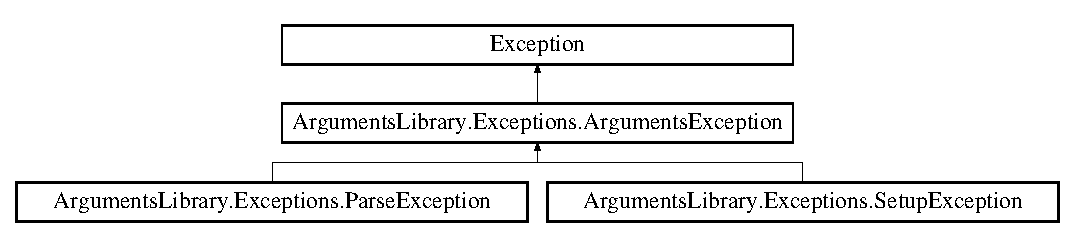
\includegraphics[height=2.754098cm]{d7/df5/class_arguments_library_1_1_exceptions_1_1_arguments_exception}
\end{center}
\end{figure}


\subsection{Detailed Description}
This is a base layer exception for \hyperlink{class_arguments_library_1_1_arguments}{Arguments} library exceptions 



The documentation for this class was generated from the following file\+:\begin{DoxyCompactItemize}
\item 
Arguments\+Library/\+Exceptions/Arguments\+Exception.\+cs\end{DoxyCompactItemize}

\hypertarget{class_arguments_library_1_1_command_line}{\section{Arguments\+Library.\+Command\+Line Class Reference}
\label{class_arguments_library_1_1_command_line}\index{Arguments\+Library.\+Command\+Line@{Arguments\+Library.\+Command\+Line}}
}
\subsection*{Public Member Functions}
\begin{DoxyCompactItemize}
\item 
bool \hyperlink{class_arguments_library_1_1_command_line_a62b6a2c027671fc637ed93347ed5ac98}{Is\+Option\+Set} (string alias)
\begin{DoxyCompactList}\small\item\em Checks whether the user specified an option or not. \end{DoxyCompactList}\item 
T \hyperlink{class_arguments_library_1_1_command_line_a23016d054a9fd5aa9de8358cba644206}{Get\+Option\+Value$<$ T $>$} (string alias)
\begin{DoxyCompactList}\small\item\em Gets Option argument converted to the specified type. \end{DoxyCompactList}\item 
string \hyperlink{class_arguments_library_1_1_command_line_ae57ef7960f96f48de5d58794bae5cdbf}{Get\+Option\+Value} (string alias)
\begin{DoxyCompactList}\small\item\em Gets Option argument as string. Same as Get\+Option\+Value\{\+T\}, implicitly typed. \end{DoxyCompactList}\item 
\hypertarget{class_arguments_library_1_1_command_line_ac554dc3a56ba1a7565a2f4b44a1cb659}{I\+Enumerable$<$ T $>$ {\bfseries Get\+Plain\+Arguments$<$ T $>$} ()}\label{class_arguments_library_1_1_command_line_ac554dc3a56ba1a7565a2f4b44a1cb659}

\item 
I\+Enumerable$<$ string $>$ \hyperlink{class_arguments_library_1_1_command_line_ac4f5141de6dbbddef9e44bbf6b725bfc}{Get\+Plain\+Arguments} ()
\begin{DoxyCompactList}\small\item\em Implicit alternative to Get\+Plain\+Arguments\{\+T\}. Returns a list of all arguments that do not correspond to Options as a list of strings. \end{DoxyCompactList}\end{DoxyCompactItemize}


\subsection{Member Function Documentation}
\hypertarget{class_arguments_library_1_1_command_line_ae57ef7960f96f48de5d58794bae5cdbf}{\index{Arguments\+Library\+::\+Command\+Line@{Arguments\+Library\+::\+Command\+Line}!Get\+Option\+Value@{Get\+Option\+Value}}
\index{Get\+Option\+Value@{Get\+Option\+Value}!Arguments\+Library\+::\+Command\+Line@{Arguments\+Library\+::\+Command\+Line}}
\subsubsection[{Get\+Option\+Value}]{\setlength{\rightskip}{0pt plus 5cm}string Arguments\+Library.\+Command\+Line.\+Get\+Option\+Value (
\begin{DoxyParamCaption}
\item[{string}]{alias}
\end{DoxyParamCaption}
)\hspace{0.3cm}{\ttfamily [inline]}}}\label{class_arguments_library_1_1_command_line_ae57ef7960f96f48de5d58794bae5cdbf}


Gets Option argument as string. Same as Get\+Option\+Value\{\+T\}, implicitly typed. 


\begin{DoxyParams}{Parameters}
{\em alias} & One of the Option aliases\\
\hline
\end{DoxyParams}
\begin{DoxyReturn}{Returns}
Option value as string
\end{DoxyReturn}
\hypertarget{class_arguments_library_1_1_command_line_a23016d054a9fd5aa9de8358cba644206}{\index{Arguments\+Library\+::\+Command\+Line@{Arguments\+Library\+::\+Command\+Line}!Get\+Option\+Value$<$ T $>$@{Get\+Option\+Value$<$ T $>$}}
\index{Get\+Option\+Value$<$ T $>$@{Get\+Option\+Value$<$ T $>$}!Arguments\+Library\+::\+Command\+Line@{Arguments\+Library\+::\+Command\+Line}}
\subsubsection[{Get\+Option\+Value$<$ T $>$}]{\setlength{\rightskip}{0pt plus 5cm}T {\bf Arguments\+Library.\+Command\+Line.\+Get\+Option\+Value}$<$ T $>$ (
\begin{DoxyParamCaption}
\item[{string}]{alias}
\end{DoxyParamCaption}
)\hspace{0.3cm}{\ttfamily [inline]}}}\label{class_arguments_library_1_1_command_line_a23016d054a9fd5aa9de8358cba644206}


Gets Option argument converted to the specified type. 


\begin{DoxyTemplParams}{Template Parameters}
{\em T} & Return type of the value\\
\hline
\end{DoxyTemplParams}

\begin{DoxyParams}{Parameters}
{\em alias} & One of the Option aliases\\
\hline
\end{DoxyParams}
\begin{DoxyReturn}{Returns}
Typed Option value
\end{DoxyReturn}
\hypertarget{class_arguments_library_1_1_command_line_ac4f5141de6dbbddef9e44bbf6b725bfc}{\index{Arguments\+Library\+::\+Command\+Line@{Arguments\+Library\+::\+Command\+Line}!Get\+Plain\+Arguments@{Get\+Plain\+Arguments}}
\index{Get\+Plain\+Arguments@{Get\+Plain\+Arguments}!Arguments\+Library\+::\+Command\+Line@{Arguments\+Library\+::\+Command\+Line}}
\subsubsection[{Get\+Plain\+Arguments}]{\setlength{\rightskip}{0pt plus 5cm}I\+Enumerable$<$string$>$ Arguments\+Library.\+Command\+Line.\+Get\+Plain\+Arguments (
\begin{DoxyParamCaption}
{}
\end{DoxyParamCaption}
)\hspace{0.3cm}{\ttfamily [inline]}}}\label{class_arguments_library_1_1_command_line_ac4f5141de6dbbddef9e44bbf6b725bfc}


Implicit alternative to Get\+Plain\+Arguments\{\+T\}. Returns a list of all arguments that do not correspond to Options as a list of strings. 

\begin{DoxyReturn}{Returns}
List of all plain arguments
\end{DoxyReturn}
\hypertarget{class_arguments_library_1_1_command_line_a62b6a2c027671fc637ed93347ed5ac98}{\index{Arguments\+Library\+::\+Command\+Line@{Arguments\+Library\+::\+Command\+Line}!Is\+Option\+Set@{Is\+Option\+Set}}
\index{Is\+Option\+Set@{Is\+Option\+Set}!Arguments\+Library\+::\+Command\+Line@{Arguments\+Library\+::\+Command\+Line}}
\subsubsection[{Is\+Option\+Set}]{\setlength{\rightskip}{0pt plus 5cm}bool Arguments\+Library.\+Command\+Line.\+Is\+Option\+Set (
\begin{DoxyParamCaption}
\item[{string}]{alias}
\end{DoxyParamCaption}
)\hspace{0.3cm}{\ttfamily [inline]}}}\label{class_arguments_library_1_1_command_line_a62b6a2c027671fc637ed93347ed5ac98}


Checks whether the user specified an option or not. 


\begin{DoxyParams}{Parameters}
{\em alias} & \\
\hline
\end{DoxyParams}
\begin{DoxyReturn}{Returns}
True if user specified an option or if a default value is defined
\end{DoxyReturn}


The documentation for this class was generated from the following file\+:\begin{DoxyCompactItemize}
\item 
Arguments\+Library/Command\+Line.\+cs\end{DoxyCompactItemize}

\hypertarget{class_arguments_library_1_1_builders_1_1_option_builder}{\section{Arguments\+Library.\+Builders.\+Option\+Builder Class Reference}
\label{class_arguments_library_1_1_builders_1_1_option_builder}\index{Arguments\+Library.\+Builders.\+Option\+Builder@{Arguments\+Library.\+Builders.\+Option\+Builder}}
}


Fluent interface provider for building Options  


\subsection*{Public Member Functions}
\begin{DoxyCompactItemize}
\item 
\hyperlink{class_arguments_library_1_1_builders_1_1_option_builder}{Option\+Builder} \hyperlink{class_arguments_library_1_1_builders_1_1_option_builder_a08da2ea4bd719448640417e4f7f70032}{Set\+Mandatory} (bool flag=true)
\begin{DoxyCompactList}\small\item\em Sets an indicator whether the Option is mandatory or not. \end{DoxyCompactList}\item 
\hyperlink{class_arguments_library_1_1_builders_1_1_option_builder}{Option\+Builder} \hyperlink{class_arguments_library_1_1_builders_1_1_option_builder_a4e67ec2746aa2f841a2da941664c2120}{With\+Aliases} (string aliases)
\begin{DoxyCompactList}\small\item\em Adds aliases to current Option, same as \hyperlink{class_arguments_library_1_1_builders_1_1_option_builder_ac04774a8724bcdfaacce9fd47d23322b}{With\+Alias} \end{DoxyCompactList}\item 
\hyperlink{class_arguments_library_1_1_builders_1_1_option_builder}{Option\+Builder} \hyperlink{class_arguments_library_1_1_builders_1_1_option_builder_ac04774a8724bcdfaacce9fd47d23322b}{With\+Alias} (string alias)
\begin{DoxyCompactList}\small\item\em Adds aliases to current Option, same as \hyperlink{class_arguments_library_1_1_builders_1_1_option_builder_a4e67ec2746aa2f841a2da941664c2120}{With\+Aliases} \end{DoxyCompactList}\item 
\hyperlink{class_arguments_library_1_1_builders_1_1_option_builder}{Option\+Builder} \hyperlink{class_arguments_library_1_1_builders_1_1_option_builder_acf6d150980aab12d911b78892562136f}{With\+Description} (string description)
\begin{DoxyCompactList}\small\item\em Description of the Option to be used when showing help \end{DoxyCompactList}\item 
\hyperlink{class_arguments_library_1_1_builders_1_1_option_builder}{Option\+Builder} \hyperlink{class_arguments_library_1_1_builders_1_1_option_builder_ad72ffd5950e6c2d5d67baa8c07545f4e}{With\+Action} (Action action)
\begin{DoxyCompactList}\small\item\em Adds an Action to be called when the Option is detected among console input arguments. Multiple actions can be specified. \end{DoxyCompactList}\item 
Argument\+Builder$<$ T $>$ \hyperlink{class_arguments_library_1_1_builders_1_1_option_builder_a7ef1bfac45f048ca3f694079db784821}{With\+Argument$<$ T $>$} (string name)
\begin{DoxyCompactList}\small\item\em Defines the Option Argument with specific type and name. \end{DoxyCompactList}\item 
Argument\+Builder$<$ string $>$ \hyperlink{class_arguments_library_1_1_builders_1_1_option_builder_a994274983f42d7a8a4a3f00a928ce50b}{With\+Argument} (string name)
\begin{DoxyCompactList}\small\item\em Same as With\+Argument\{\+T\}, implicitly typed as string. \end{DoxyCompactList}\item 
Argument\+Builder$<$ T $>$ \hyperlink{class_arguments_library_1_1_builders_1_1_option_builder_a671ec77a1bf3044a86242966c5b492cc}{With\+Optional\+Argument$<$ T $>$} (string name)
\begin{DoxyCompactList}\small\item\em Defines an optional Argument Same as With\+Argument\{\+T\}, \end{DoxyCompactList}\item 
Argument\+Builder$<$ string $>$ \hyperlink{class_arguments_library_1_1_builders_1_1_option_builder_aaed523e2969b04dcb2757f730bc1a06b}{With\+Optional\+Argument} (string name)
\begin{DoxyCompactList}\small\item\em Same as With\+Optional\+Argument\{\+T\}, implicitly typed as string\end{DoxyCompactList}\end{DoxyCompactItemize}


\subsection{Detailed Description}
Fluent interface provider for building Options 



\subsection{Member Function Documentation}
\hypertarget{class_arguments_library_1_1_builders_1_1_option_builder_a08da2ea4bd719448640417e4f7f70032}{\index{Arguments\+Library\+::\+Builders\+::\+Option\+Builder@{Arguments\+Library\+::\+Builders\+::\+Option\+Builder}!Set\+Mandatory@{Set\+Mandatory}}
\index{Set\+Mandatory@{Set\+Mandatory}!Arguments\+Library\+::\+Builders\+::\+Option\+Builder@{Arguments\+Library\+::\+Builders\+::\+Option\+Builder}}
\subsubsection[{Set\+Mandatory}]{\setlength{\rightskip}{0pt plus 5cm}{\bf Option\+Builder} Arguments\+Library.\+Builders.\+Option\+Builder.\+Set\+Mandatory (
\begin{DoxyParamCaption}
\item[{bool}]{flag = {\ttfamily true}}
\end{DoxyParamCaption}
)\hspace{0.3cm}{\ttfamily [inline]}}}\label{class_arguments_library_1_1_builders_1_1_option_builder_a08da2ea4bd719448640417e4f7f70032}


Sets an indicator whether the Option is mandatory or not. 


\begin{DoxyParams}{Parameters}
{\em flag} & True if mandatory, False otherwise\\
\hline
\end{DoxyParams}
\begin{DoxyReturn}{Returns}

\end{DoxyReturn}
\hypertarget{class_arguments_library_1_1_builders_1_1_option_builder_ad72ffd5950e6c2d5d67baa8c07545f4e}{\index{Arguments\+Library\+::\+Builders\+::\+Option\+Builder@{Arguments\+Library\+::\+Builders\+::\+Option\+Builder}!With\+Action@{With\+Action}}
\index{With\+Action@{With\+Action}!Arguments\+Library\+::\+Builders\+::\+Option\+Builder@{Arguments\+Library\+::\+Builders\+::\+Option\+Builder}}
\subsubsection[{With\+Action}]{\setlength{\rightskip}{0pt plus 5cm}{\bf Option\+Builder} Arguments\+Library.\+Builders.\+Option\+Builder.\+With\+Action (
\begin{DoxyParamCaption}
\item[{Action}]{action}
\end{DoxyParamCaption}
)\hspace{0.3cm}{\ttfamily [inline]}}}\label{class_arguments_library_1_1_builders_1_1_option_builder_ad72ffd5950e6c2d5d67baa8c07545f4e}


Adds an Action to be called when the Option is detected among console input arguments. Multiple actions can be specified. 


\begin{DoxyParams}{Parameters}
{\em action} & Action to be performed when the Option is detected among input arguments\\
\hline
\end{DoxyParams}
\begin{DoxyReturn}{Returns}
\hyperlink{class_arguments_library_1_1_builders_1_1_option_builder}{Option\+Builder} fluent interface
\end{DoxyReturn}
\hypertarget{class_arguments_library_1_1_builders_1_1_option_builder_ac04774a8724bcdfaacce9fd47d23322b}{\index{Arguments\+Library\+::\+Builders\+::\+Option\+Builder@{Arguments\+Library\+::\+Builders\+::\+Option\+Builder}!With\+Alias@{With\+Alias}}
\index{With\+Alias@{With\+Alias}!Arguments\+Library\+::\+Builders\+::\+Option\+Builder@{Arguments\+Library\+::\+Builders\+::\+Option\+Builder}}
\subsubsection[{With\+Alias}]{\setlength{\rightskip}{0pt plus 5cm}{\bf Option\+Builder} Arguments\+Library.\+Builders.\+Option\+Builder.\+With\+Alias (
\begin{DoxyParamCaption}
\item[{string}]{alias}
\end{DoxyParamCaption}
)\hspace{0.3cm}{\ttfamily [inline]}}}\label{class_arguments_library_1_1_builders_1_1_option_builder_ac04774a8724bcdfaacce9fd47d23322b}


Adds aliases to current Option, same as \hyperlink{class_arguments_library_1_1_builders_1_1_option_builder_a4e67ec2746aa2f841a2da941664c2120}{With\+Aliases} 


\begin{DoxyParams}{Parameters}
{\em alias} & One or more aliases\\
\hline
\end{DoxyParams}
\begin{DoxyReturn}{Returns}
\hyperlink{class_arguments_library_1_1_builders_1_1_option_builder}{Option\+Builder} fluent interface
\end{DoxyReturn}
\hypertarget{class_arguments_library_1_1_builders_1_1_option_builder_a4e67ec2746aa2f841a2da941664c2120}{\index{Arguments\+Library\+::\+Builders\+::\+Option\+Builder@{Arguments\+Library\+::\+Builders\+::\+Option\+Builder}!With\+Aliases@{With\+Aliases}}
\index{With\+Aliases@{With\+Aliases}!Arguments\+Library\+::\+Builders\+::\+Option\+Builder@{Arguments\+Library\+::\+Builders\+::\+Option\+Builder}}
\subsubsection[{With\+Aliases}]{\setlength{\rightskip}{0pt plus 5cm}{\bf Option\+Builder} Arguments\+Library.\+Builders.\+Option\+Builder.\+With\+Aliases (
\begin{DoxyParamCaption}
\item[{string}]{aliases}
\end{DoxyParamCaption}
)\hspace{0.3cm}{\ttfamily [inline]}}}\label{class_arguments_library_1_1_builders_1_1_option_builder_a4e67ec2746aa2f841a2da941664c2120}


Adds aliases to current Option, same as \hyperlink{class_arguments_library_1_1_builders_1_1_option_builder_ac04774a8724bcdfaacce9fd47d23322b}{With\+Alias} 


\begin{DoxyParams}{Parameters}
{\em aliases} & One or more aliases\\
\hline
\end{DoxyParams}
\begin{DoxyReturn}{Returns}
\hyperlink{class_arguments_library_1_1_builders_1_1_option_builder}{Option\+Builder} fluent interface
\end{DoxyReturn}
\hypertarget{class_arguments_library_1_1_builders_1_1_option_builder_a994274983f42d7a8a4a3f00a928ce50b}{\index{Arguments\+Library\+::\+Builders\+::\+Option\+Builder@{Arguments\+Library\+::\+Builders\+::\+Option\+Builder}!With\+Argument@{With\+Argument}}
\index{With\+Argument@{With\+Argument}!Arguments\+Library\+::\+Builders\+::\+Option\+Builder@{Arguments\+Library\+::\+Builders\+::\+Option\+Builder}}
\subsubsection[{With\+Argument}]{\setlength{\rightskip}{0pt plus 5cm}Argument\+Builder$<$string$>$ Arguments\+Library.\+Builders.\+Option\+Builder.\+With\+Argument (
\begin{DoxyParamCaption}
\item[{string}]{name}
\end{DoxyParamCaption}
)\hspace{0.3cm}{\ttfamily [inline]}}}\label{class_arguments_library_1_1_builders_1_1_option_builder_a994274983f42d7a8a4a3f00a928ce50b}


Same as With\+Argument\{\+T\}, implicitly typed as string. 


\begin{DoxyParams}{Parameters}
{\em name} & Name of the argument to be used in help\\
\hline
\end{DoxyParams}
\begin{DoxyReturn}{Returns}
Argument\+Builder\{string\} fluent interface
\end{DoxyReturn}
\hypertarget{class_arguments_library_1_1_builders_1_1_option_builder_a7ef1bfac45f048ca3f694079db784821}{\index{Arguments\+Library\+::\+Builders\+::\+Option\+Builder@{Arguments\+Library\+::\+Builders\+::\+Option\+Builder}!With\+Argument$<$ T $>$@{With\+Argument$<$ T $>$}}
\index{With\+Argument$<$ T $>$@{With\+Argument$<$ T $>$}!Arguments\+Library\+::\+Builders\+::\+Option\+Builder@{Arguments\+Library\+::\+Builders\+::\+Option\+Builder}}
\subsubsection[{With\+Argument$<$ T $>$}]{\setlength{\rightskip}{0pt plus 5cm}Argument\+Builder$<$T$>$ {\bf Arguments\+Library.\+Builders.\+Option\+Builder.\+With\+Argument}$<$ T $>$ (
\begin{DoxyParamCaption}
\item[{string}]{name}
\end{DoxyParamCaption}
)\hspace{0.3cm}{\ttfamily [inline]}}}\label{class_arguments_library_1_1_builders_1_1_option_builder_a7ef1bfac45f048ca3f694079db784821}


Defines the Option Argument with specific type and name. 


\begin{DoxyTemplParams}{Template Parameters}
{\em T} & Type of the Option Argument\\
\hline
\end{DoxyTemplParams}

\begin{DoxyParams}{Parameters}
{\em name} & Name of the argument to be used in help\\
\hline
\end{DoxyParams}
\begin{DoxyReturn}{Returns}
Argument\+Builder\{T\} fluent interface
\end{DoxyReturn}
\hypertarget{class_arguments_library_1_1_builders_1_1_option_builder_acf6d150980aab12d911b78892562136f}{\index{Arguments\+Library\+::\+Builders\+::\+Option\+Builder@{Arguments\+Library\+::\+Builders\+::\+Option\+Builder}!With\+Description@{With\+Description}}
\index{With\+Description@{With\+Description}!Arguments\+Library\+::\+Builders\+::\+Option\+Builder@{Arguments\+Library\+::\+Builders\+::\+Option\+Builder}}
\subsubsection[{With\+Description}]{\setlength{\rightskip}{0pt plus 5cm}{\bf Option\+Builder} Arguments\+Library.\+Builders.\+Option\+Builder.\+With\+Description (
\begin{DoxyParamCaption}
\item[{string}]{description}
\end{DoxyParamCaption}
)\hspace{0.3cm}{\ttfamily [inline]}}}\label{class_arguments_library_1_1_builders_1_1_option_builder_acf6d150980aab12d911b78892562136f}


Description of the Option to be used when showing help 


\begin{DoxyParams}{Parameters}
{\em description} & \\
\hline
\end{DoxyParams}
\begin{DoxyReturn}{Returns}
\hyperlink{class_arguments_library_1_1_builders_1_1_option_builder}{Option\+Builder} fluent interface
\end{DoxyReturn}
\hypertarget{class_arguments_library_1_1_builders_1_1_option_builder_aaed523e2969b04dcb2757f730bc1a06b}{\index{Arguments\+Library\+::\+Builders\+::\+Option\+Builder@{Arguments\+Library\+::\+Builders\+::\+Option\+Builder}!With\+Optional\+Argument@{With\+Optional\+Argument}}
\index{With\+Optional\+Argument@{With\+Optional\+Argument}!Arguments\+Library\+::\+Builders\+::\+Option\+Builder@{Arguments\+Library\+::\+Builders\+::\+Option\+Builder}}
\subsubsection[{With\+Optional\+Argument}]{\setlength{\rightskip}{0pt plus 5cm}Argument\+Builder$<$string$>$ Arguments\+Library.\+Builders.\+Option\+Builder.\+With\+Optional\+Argument (
\begin{DoxyParamCaption}
\item[{string}]{name}
\end{DoxyParamCaption}
)\hspace{0.3cm}{\ttfamily [inline]}}}\label{class_arguments_library_1_1_builders_1_1_option_builder_aaed523e2969b04dcb2757f730bc1a06b}


Same as With\+Optional\+Argument\{\+T\}, implicitly typed as string


\begin{DoxyParams}{Parameters}
{\em name} & Name of the argument to be used in help\\
\hline
\end{DoxyParams}
\begin{DoxyReturn}{Returns}
Argument\+Builder\{string\} fluent interface
\end{DoxyReturn}
\hypertarget{class_arguments_library_1_1_builders_1_1_option_builder_a671ec77a1bf3044a86242966c5b492cc}{\index{Arguments\+Library\+::\+Builders\+::\+Option\+Builder@{Arguments\+Library\+::\+Builders\+::\+Option\+Builder}!With\+Optional\+Argument$<$ T $>$@{With\+Optional\+Argument$<$ T $>$}}
\index{With\+Optional\+Argument$<$ T $>$@{With\+Optional\+Argument$<$ T $>$}!Arguments\+Library\+::\+Builders\+::\+Option\+Builder@{Arguments\+Library\+::\+Builders\+::\+Option\+Builder}}
\subsubsection[{With\+Optional\+Argument$<$ T $>$}]{\setlength{\rightskip}{0pt plus 5cm}Argument\+Builder$<$T$>$ {\bf Arguments\+Library.\+Builders.\+Option\+Builder.\+With\+Optional\+Argument}$<$ T $>$ (
\begin{DoxyParamCaption}
\item[{string}]{name}
\end{DoxyParamCaption}
)\hspace{0.3cm}{\ttfamily [inline]}}}\label{class_arguments_library_1_1_builders_1_1_option_builder_a671ec77a1bf3044a86242966c5b492cc}


Defines an optional Argument Same as With\+Argument\{\+T\}, 


\begin{DoxyTemplParams}{Template Parameters}
{\em T} & Type of the Option Argument\\
\hline
\end{DoxyTemplParams}

\begin{DoxyParams}{Parameters}
{\em name} & Name of the argument to be used in help\\
\hline
\end{DoxyParams}
\begin{DoxyReturn}{Returns}
Argument\+Builder\{T\} fluent interface
\end{DoxyReturn}


The documentation for this class was generated from the following file\+:\begin{DoxyCompactItemize}
\item 
Arguments\+Library/\+Builders/Option\+Builder.\+cs\end{DoxyCompactItemize}

\hypertarget{class_arguments_library_1_1_exceptions_1_1_parse_exception}{\section{Arguments\+Library.\+Exceptions.\+Parse\+Exception Class Reference}
\label{class_arguments_library_1_1_exceptions_1_1_parse_exception}\index{Arguments\+Library.\+Exceptions.\+Parse\+Exception@{Arguments\+Library.\+Exceptions.\+Parse\+Exception}}
}


Exception thrown during \hyperlink{class_arguments_library_1_1_arguments}{Arguments} parse phase when invalid command line input is detected  


Inheritance diagram for Arguments\+Library.\+Exceptions.\+Parse\+Exception\+:\begin{figure}[H]
\begin{center}
\leavevmode
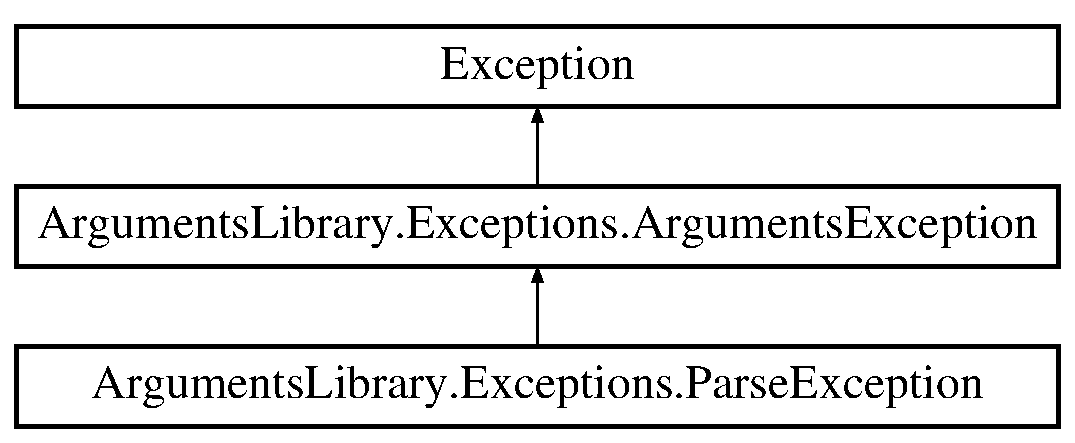
\includegraphics[height=3.000000cm]{da/dd1/class_arguments_library_1_1_exceptions_1_1_parse_exception}
\end{center}
\end{figure}


\subsection{Detailed Description}
Exception thrown during \hyperlink{class_arguments_library_1_1_arguments}{Arguments} parse phase when invalid command line input is detected 



The documentation for this class was generated from the following file\+:\begin{DoxyCompactItemize}
\item 
Arguments\+Library/\+Exceptions/Parse\+Exception.\+cs\end{DoxyCompactItemize}

\hypertarget{class_arguments_library_1_1_exceptions_1_1_setup_exception}{\section{Arguments\+Library.\+Exceptions.\+Setup\+Exception Class Reference}
\label{class_arguments_library_1_1_exceptions_1_1_setup_exception}\index{Arguments\+Library.\+Exceptions.\+Setup\+Exception@{Arguments\+Library.\+Exceptions.\+Setup\+Exception}}
}


Exception thrown during \hyperlink{class_arguments_library_1_1_arguments}{Arguments} setup phase when invalid setup is detected  


Inheritance diagram for Arguments\+Library.\+Exceptions.\+Setup\+Exception\+:\begin{figure}[H]
\begin{center}
\leavevmode
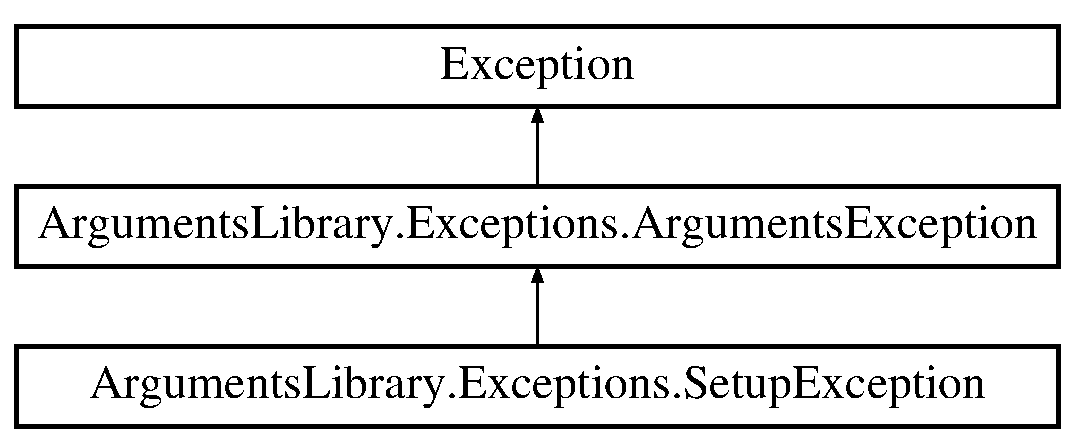
\includegraphics[height=3.000000cm]{d1/d04/class_arguments_library_1_1_exceptions_1_1_setup_exception}
\end{center}
\end{figure}


\subsection{Detailed Description}
Exception thrown during \hyperlink{class_arguments_library_1_1_arguments}{Arguments} setup phase when invalid setup is detected 



The documentation for this class was generated from the following file\+:\begin{DoxyCompactItemize}
\item 
Arguments\+Library/\+Exceptions/Setup\+Exception.\+cs\end{DoxyCompactItemize}

%--- End generated contents ---

% Index
\newpage
\phantomsection
\addcontentsline{toc}{chapter}{Index}
\printindex

\end{document}
